\chapter{Introduction \& Motivation}\label{chap:motivation}
Understanding the properties of Strongly Correlated Quantum Systems is a cornerstone of modern physics research. Experimental and theoretical studies of such systems range from ultracold atoms to the hot phases of the Early Universe and from the non-perturbative infrared sector of Quantum Chromodynamics (QCD) to  ultraviolet completions of the Standard Model of Particle Physics and possible connections to the realization of a theory of Quantum Gravity in Nature.\\
This thesis focuses particularly on the infrared regime of QCD, the theory of strong interactions, describing the physics of quarks and gluons, the fundamental constituents of atomic nuclei. The strong interaction being  one of the four fundamental forces, QCD is embedded in the framework of the Standard Model of Particle Physics, hence is of particular importance for fundamental physics. From a theorist's point of view, the Standard Model is the most general renormalizable field theory with gauge group 
\begin{equation}
	G_{\text{SM}} = SU(3)\otimes SU(2) \otimes U(1),
\end{equation}
three generations of fermions, and a scalar \cite{Hebecker2020}. Here, the pure gauge part of QCD contributes via the non-Abelian $SU(3)$ color group. This description of the gluonic sector in terms of a non-Abelian gauge theory goes back to the pioneering work of Yang and Mills in 1954 \cite{YangMills1954}, hence it is usually referred to as Yang-Mills theory.     \\
Understanding the infrared dynamics of the Yang-Mills sector of QCD is directly linked to the most pressing open questions in QCD, for an overview cf. \cite{Brambilla2014}. Maybe the most prominent example is the phenomenon of confinement, i.\,e. that the theory features a mass gap\footnote{The mathematical proof of the existence of a mass gapped quantum Yang-Mills theory has even been declared as one of the seven Millennium Prize Problems \cite{JaffeWitten2009}.} and that quarks and gluons can only be observed as color-neutral bound states, called hadrons \cite{vonSmekalAlkoferHauck1997, AlkoferVonSmekal2000, LercheVonSmekal2002, FischerMaasPawlowski2008,CyrolFisterMitterPawlowskiStrodthoff2016}. The associated temperature of the so-called confinement-deconfinement transition, i.\,e. the transition between the confined phase and a state of matter called the Quark-Gluon Plasma (QGP), where the deconfined quarks and gluons are the relevant degrees of freedom, has been determined in lattice studies to be of the order of $T\approx 155$ MeV \cite{AokiFodorKatzSzabo2006}. The phenomenologically rich hadron spectrum makes up a large fraction of all observed matter around us and has been subject of many experimental and theoretical investigations during the last decades.\\ Open questions in the matter sector of QCD include for example the understanding of resonant four-quark interactions \cite{Eichmann2020}, directly connected to the beforehand mentioned variety in the hadronic spectrum and spontaneous chiral symmetry breaking \cite{MitterPawlowskiStrodthoff2014}, the mechanism behind mass generation of nucleons from much lighter quarks. This is usually investigated in low-energy effective models such as Nambu-Jona-Lasinio (NJL) or Quark-Meson (QM) models \cite{NambuJonaLasinio1961, Tetradis2003}. \\ 
\begin{figure}[t]
\centering
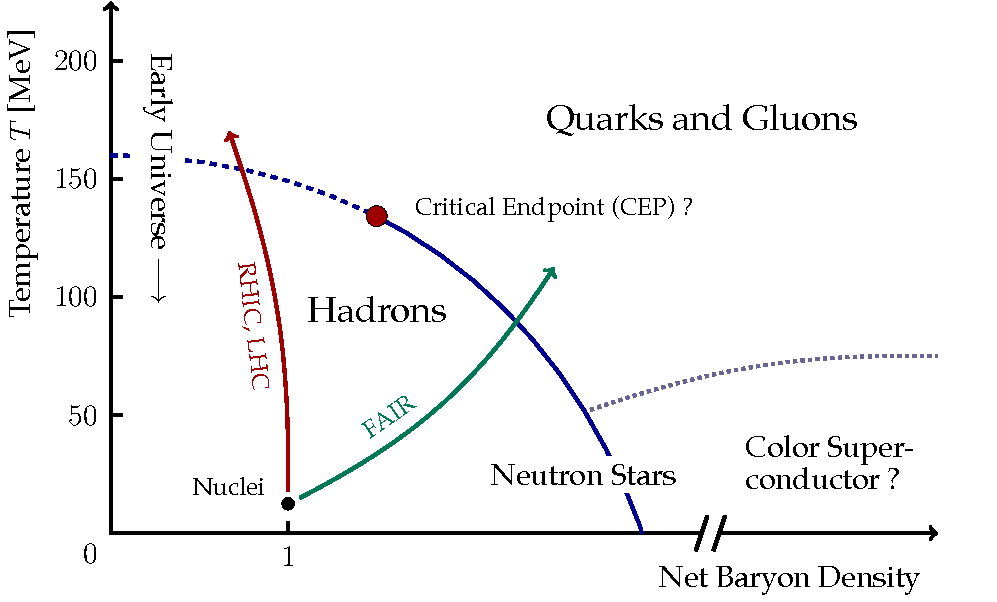
\includegraphics[width=0.8\textwidth]{figs/tikz/qcd_phase_diagram}
\caption[Schematic sketch of the QCD phase diagram.]{Schematic sketch of the QCD phase diagram, inspired by the graphic provided by the GSI/Darmstadt. The dashed blue curve signals a second order phase transition, the solid blue curve the (possible) first order transition regime. The red and green lines indicate the respective areas of the diagram that are tested by experiments at the moment or in the near future, cf. \cite{RHIC, LHC, FAIR, NICA}.}\label{fig:phase_diagram}
\end{figure}
\hspace{-0.5em}Another major task is to obtain a comprehensive understanding of the full QCD phase diagram at finite temperature and baryon density  \cite{Wink2020, BraunHaasMarhauserPawlowski2009,FuPawlowskiRennecke2019}, cf. \figref{fig:phase_diagram} for a schematic overview. Current debates focus for example on the question whether there exists a critical endpoint (CEP) \cite{AokiFodorKatzSzabo2006}. \\
On the technical side, our theoretical understanding of the non-perturbative sector of QCD from first principles has greatly improved during the last decades, mainly due to complementary efforts and advances in the application  of lattice techniques \cite{Philipsen2007, deForcrand2010} and  Functional Methods such as the Functional Renormalization Group (FRG), cf. \cite{Wetterich1992, Pawlowski2005, Dupuis2020} for general reviews, and \cite{NPgaugeLecture} for various applications in QCD (and Gravity), Bethe-Salpeter equations \cite{BetheSalpeter1951}, or Dyson-Schwinger equations (DSEs) \cite{Dyson1949, Schwinger1951}. The latter one will be the tool of our choice throughout this work. Earlier studies of the infrared regime of QCD using DSEs were put forward for example in \cite{Fischer2006,Fischer2019, Maris2003, RobertsWilliams1994}.\\
Of course, there have also been many advances on the experimental side, where the phase diagram is usually studied in the context of relativistic heavy-ion collisions at collider facilities such as the Relativistic Heavy-Ion Collider (RHIC) at the Brookhaven National Lab \cite{RHIC} and the Large Hadron Collider (LHC) at CERN in Geneva \cite{LHC} and in the near future at FAIR/GSI in Darmstadt \cite{FAIR} and NICA in Dubna \cite{NICA}. \\
Nevertheless, it is far from trivial to map measured signatures directly to certain points in the phase diagram. This is due to the fact, that the phase diagram is associated with equilibrium, which is definitely not realized in the initial stages of heavy-ion collisions. Understanding the thermalization process, i.\,e. the stage at which the system approaches thermal equilibrium, is therefore key to be able to connect the measured signatures to theoretical predictions. But this is still a subject of ongoing research efforts, cf. \cite{Blaizot2012, Blaizot2016, Wolschin2020, SchlichtingTeaney2019}.\\
To conclude this overview, we should remark, that all these different methods suffer from technical limitations and are therefore only applicable in specific regions of the phase diagram. Certainly, one should not forget the contributions from perturbation theory (PT) that had great impact on the development of the theory, cf. \cite{EllisGeorgiMachacekPolitzerRoss1979,BernardGolterman1992}, but in in the infrared sector, PT is not applicable since it is usually based on expansions in terms of small coupling constants, which is in conflict with the observation of asymptotic freedom, i.\,e. that the gauge coupling rises extremely quick in the infrared and tends to zero in the ultraviolet. This prediction earned Gross, Politzer and Wilczek the 2004 Nobel Prize in Physics \cite{Politzer1973, GrossWilczek1973}. Lattice computations, where the idea is to discretize the continuum theory and restore the physical continuum limit by extending the lattice size and lowering the grid spacing, make solid predictions for small and vanishing chemical potential. In the region $\mu/T\gtrsim 1$, the infamous sign-problem hinders predictability \cite{Philipsen2007, deForcrand2010}. The application of functional methods is in general not affected by such inherent problems, but rather by limitations in computing power and analytic feasibility of the conducted computations. This will of course improve in the future with the ongoing developments in hardware and computer-algebra systems.\\
A pivotal ingredient in the study of Strongly Correlated Systems are real-time correlation functions since they allow us to access the real-time dynamics of the theory at hand. In the context of QCD this includes for example transport phenomena relevant in the hydrodynamical description of heavy-ion collisions as outlined above, cf. \cite{AyikNorenbergWolschin1977, Xu2019}.\\  
Despite the beforehand mentioned advances in the field, the direct computation of these real-time quantities has turned out to pose several problems, i.\,e. results can only be obtained employing specific approximation schemes. We want to tackle this challenging task by making use of the recently developed technique of Spectral Renormalization \cite{Horak2019, Wink2020, HorakPawlowskiWink2020}, allowing for the direct computation of real-time correlation functions from their respective spectral representations, based on the gauge-invariant dimensional regularization scheme.\\
In this thesis we will focus on the real-time properties of QCD, or to be more precise, on the computation of spectral functions for the quark sector and the analytic properties of the associated correlation functions, since they provide the information needed for first principle investigations of the dynamical properties of the theory.\\

 The structure of this work is as follows. In  \chapref{chap:methods} we lay the foundation for the field theoretical conventions. We employ the functional methods needed for our treatment of non-perturbative QCD including the Dyson-Schwinger equation as the central functional relation in the context of our work. A discussion of the spectral properties of the theory in terms of the K\"all\'{e}n-Lehmann spectral representation of correlation functions completes our introduction to non-perturbative quantum field theory. \chapref{chap:qcd} provides the background knowledge on the quantization of general non-Abelian gauge theories and the special case of $SU(N_c)$ Yang-Mills theory, the underlying gauge theory of QCD. Subsequently, the fermionic quark sector of QCD is discussed and the respective Dyson-Schwinger equations are presented. A detailed presentation and assessment of the methodology and our main results follow in \chapref{chap:results}. Our findings are then summarized in \chapref{chap:conclusion} and an outlook for future investigations is given. \\
The interested reader can find the technical details of the conducted calculations in \appref{chap:appendixA} and \appref{chap:appendixB} respectively. Additional comments on the numerical implementation in Mathematica can be found in \appref{chap:appendixC}.\\
 Throughout this thesis we use natural units such that $\hbar = c  \equiv 1$ and work in Euclidean spacetime  $g_{\mu\nu}=\delta_{\mu\nu}$. Einsteins sum convention is implicitly understood: Whenever an index appears twice in a single term, summation of that term over the whole index range is implied. As usual, greek indices refer to some $d$-dim. spacetime coordinates, ranging from $0$ to $d-1$, i.\,e. $x^{\mu} = (x^0, x^1, \cdots, x^{d-1})$. Vectorial quantities are typeset in boldface. Unless stated otherwise, we work in $d=4$ spacetime dimensions.
